\documentclass[11pt,a4paper]{article}

% --- Packages ---
\usepackage[utf8]{inputenc}
\usepackage[T1]{fontenc}
\usepackage{lmodern}
\usepackage[margin=2.5cm]{geometry}
\usepackage{graphicx}
\usepackage{booktabs}
\usepackage{amsmath}
\usepackage{hyperref}
\usepackage{xcolor}
\usepackage{caption}
\usepackage{subcaption}
\usepackage{float}
\usepackage{natbib}
\usepackage{enumitem}

\hypersetup{
    colorlinks=true,
    linkcolor=blue!60!black,
    citecolor=blue!60!black,
    urlcolor=blue!60!black
}

\graphicspath{{../results/figures/}}

\title{Where Does Turkish Reasoning Diverge from English Inside Llama-3-8B?\\[0.3em]
\large A Logit Lens Pilot Study}
\author{Toprak Tarkan Dikici\\
M.Sc.\ Philosophy \& Computer Science, University of Bayreuth\\
\texttt{toprakdikici28@gmail.com}}
\date{March 2026}

\begin{document}
\maketitle

\begin{abstract}
Large language models can solve math problems in English but struggle with lower-resource languages like Turkish.
We apply the \emph{logit lens} to Llama-3-8B, projecting hidden states through the unembedding matrix at every layer to track where the model forms its answer.
On 15 matched grade-school math problems from GSM8K and GSM8K-TR, we find that English and Turkish reasoning trajectories are \emph{indistinguishable} through the first 26 layers, then diverge sharply: by the final layer, P(correct answer) reaches 0.84 for English versus 0.67 for Turkish under an English prompt frame (Hedges' $g = 1.04$, $p < 0.005$).
A Turkish prompt-frame control reveals that much of this Turkish performance depends on the English prompt scaffolding---when switched to a native Turkish frame, P(answer) drops to 0.12.
Tokenization fragmentation explains only 18\% of the variance.
These results identify layers 27--32 as the critical intervention site for future activation patching experiments aimed at improving multilingual reasoning.
\end{abstract}

% ============================================================
\section{Introduction}
% ============================================================

LLMs exhibit strong mathematical reasoning in English but degrade on lower-resource languages.
Chain-of-thought prompting can even \emph{hurt} Turkish performance in weaker models \citep{yuksel2024turkishmlu}, and even GPT-4 fails at morphological compositional generalization in agglutinative languages \citep{ismayilzada2025}.
Recent work confirms that latent reasoning collapses entirely in low-resource languages for hard tasks \citep{liu2026multilingual}.

Existing evaluations measure \emph{how much} reasoning degrades across languages, but not \emph{where inside the model} the failure originates.
The \textbf{logit lens} \citep{nostalgebraist2020} offers a window into intermediate processing by projecting each layer's hidden state through the unembedding matrix to obtain a probability distribution over the vocabulary.
By tracking P(correct answer) across layers for matched English--Turkish problem pairs, we can pinpoint the exact layers where Turkish reasoning diverges.

This pilot study validates this diagnostic approach on Llama-3-8B, establishing the feasibility of mechanistic analysis for multilingual reasoning and identifying specific intervention targets for future work.
We use ``reasoning'' throughout to refer to the task-level capability (multi-step math problem-solving), not to imply deliberative search; Llama-3-8B is a standard autoregressive language model.

% ============================================================
\section{Method}
% ============================================================

\subsection{Data}

We select 15 matched problems from GSM8K \citep{cobbe2021gsm8k} (English) and GSM8K-TR\footnote{\url{https://huggingface.co/datasets/malhajar/gsm8k-tr}} (Turkish translation), aligned by index with identical numeric answers.
Problems are stratified by difficulty (2--6 reasoning steps).
Token fertility ratios (TR tokens / EN tokens) range from 0.6$\times$ to 2.7$\times$ (mean: 1.38$\times$).

\subsection{Model}

We use \textbf{Meta-Llama-3-8B} (base, 32 transformer layers) for the logit lens analysis and Llama-3-8B-Instruct for the behavioral baseline.
The base model is loaded in float16 on an A100 40GB GPU.

\subsection{Logit Lens}

For each of the 33 hidden states (embedding + 32 layers), we extract the residual stream at the last token position and project it through:
\begin{equation}
    P_\ell = \text{softmax}\!\left(\mathbf{W}_{\text{unembed}} \cdot \text{RMSNorm}(\mathbf{h}_\ell)\right)
\end{equation}
where $\mathbf{h}_\ell$ is the hidden state at layer $\ell$ and RMSNorm is the model's final normalization layer.
Applying RMSNorm before the unembedding matrix is critical for Llama-3 \citep{belrose2023tuned}.
All softmax computations use float32 to avoid numerical issues with the 128K vocabulary.

We track three quantities per layer: P(correct answer token), top-$k$ predicted tokens, and entropy of the full distribution.

\subsection{Experimental Conditions}

Each problem is run under three conditions:
\begin{enumerate}[nosep]
    \item \textbf{EN (English frame)}: English question with ``Q: \ldots A: The answer is''
    \item \textbf{TR (English frame)}: Turkish question with the same English prompt frame
    \item \textbf{TR (Turkish frame)}: Turkish question with ``Soru: \ldots Cevap:''
\end{enumerate}
Condition 3 serves as a control to disentangle prompt-frame effects from reasoning ability.

\subsection{Statistical Methods}

We use paired permutation tests (exact enumeration for $n \leq 20$) for significance testing, Hedges' $g$ for effect sizes, and Holm--Bonferroni correction for multiple comparisons across three layer regions (early: 0--10, mid: 11--21, late: 22--32).
Behavioral confidence intervals use Wilson score intervals, and Fisher's exact test compares overall accuracy.
All trajectory confidence intervals use the $t$-distribution ($t_{14, 0.025} = 2.145$), appropriate for $n = 15$.

% ============================================================
\section{Results}
% ============================================================

\subsection{Behavioral Baseline}

Using Llama-3-8B-Instruct with chain-of-thought prompting (Figure~\ref{fig:accuracy}), English achieves 33.3\% accuracy [95\% CI: 15.2--58.3\%] and Turkish 40.0\% [19.8--64.3\%].
The difference is not significant (Fisher's exact $p = 1.0$, $n = 15$).
Despite comparable behavioral performance, the logit lens reveals divergent internal processing.

\begin{figure}[H]
    \centering
    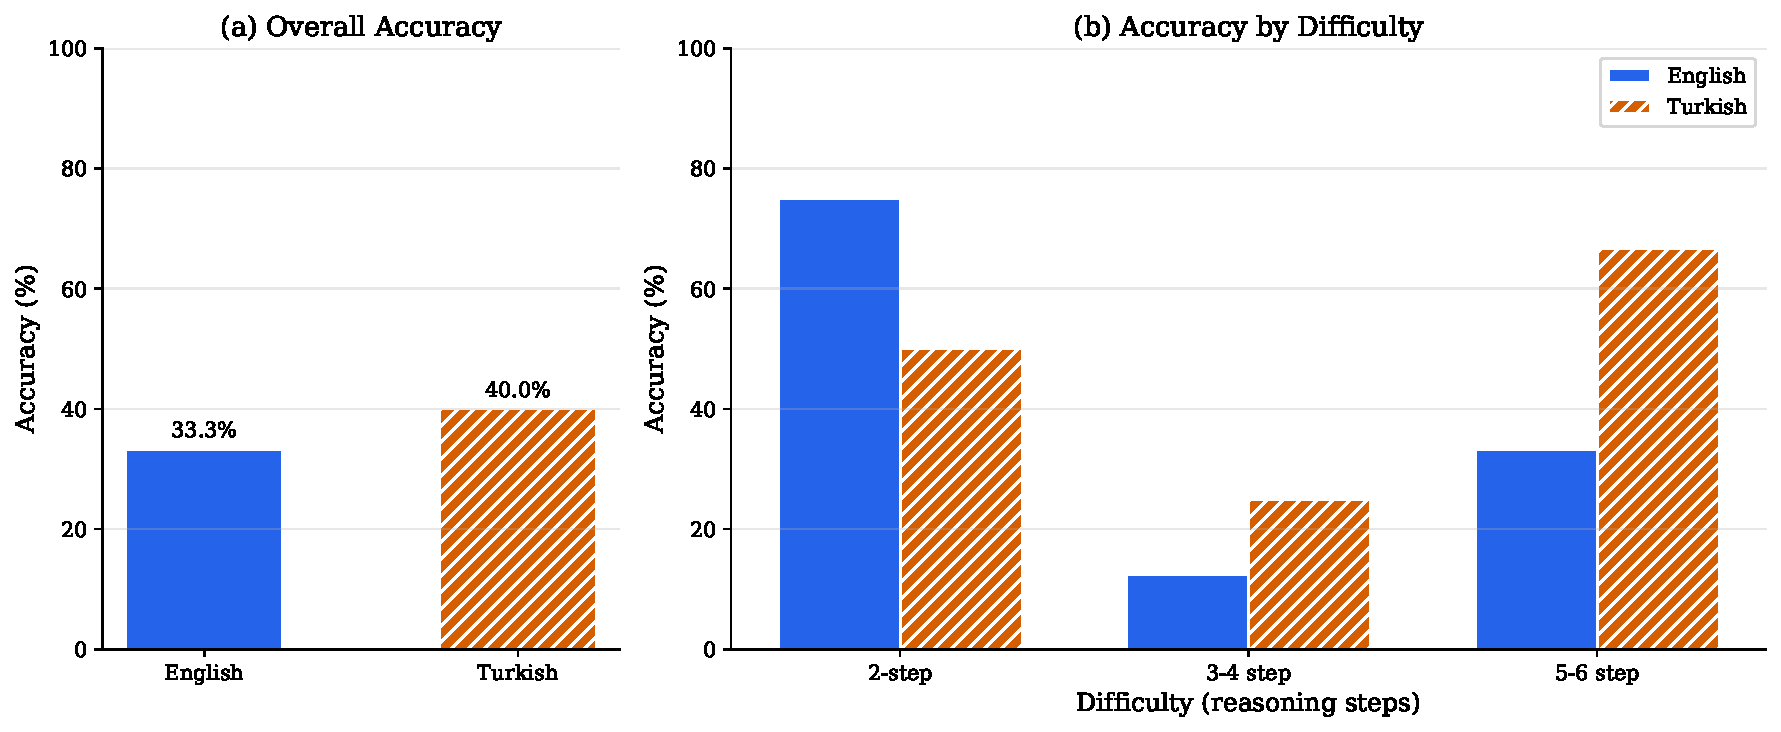
\includegraphics[width=0.85\textwidth]{fig1_accuracy_comparison.pdf}
    \caption{Behavioral accuracy of Llama-3-8B-Instruct on 15 matched GSM8K problems with Wilson 95\% CIs. (a)~Overall accuracy with Fisher's exact $p$-value. (b)~Accuracy stratified by difficulty with per-bin sample sizes. All differences are non-significant at this sample size.}
    \label{fig:accuracy}
\end{figure}

\subsection{Reasoning Trajectory Divergence}

Figure~\ref{fig:trajectory} shows the core finding.
Mean P(correct answer) is near zero for both languages through layer 26.
English then rises steeply, reaching 0.84 at the final layer, while Turkish reaches 0.67 under the English frame.
The median divergence onset is layer 27 (range: 25--32).
Note that the wide confidence intervals for English in the late layers reflect the heterogeneity across problems---some problems reach P $> 0.9$ while others remain near zero for both languages.

\begin{figure}[H]
    \centering
    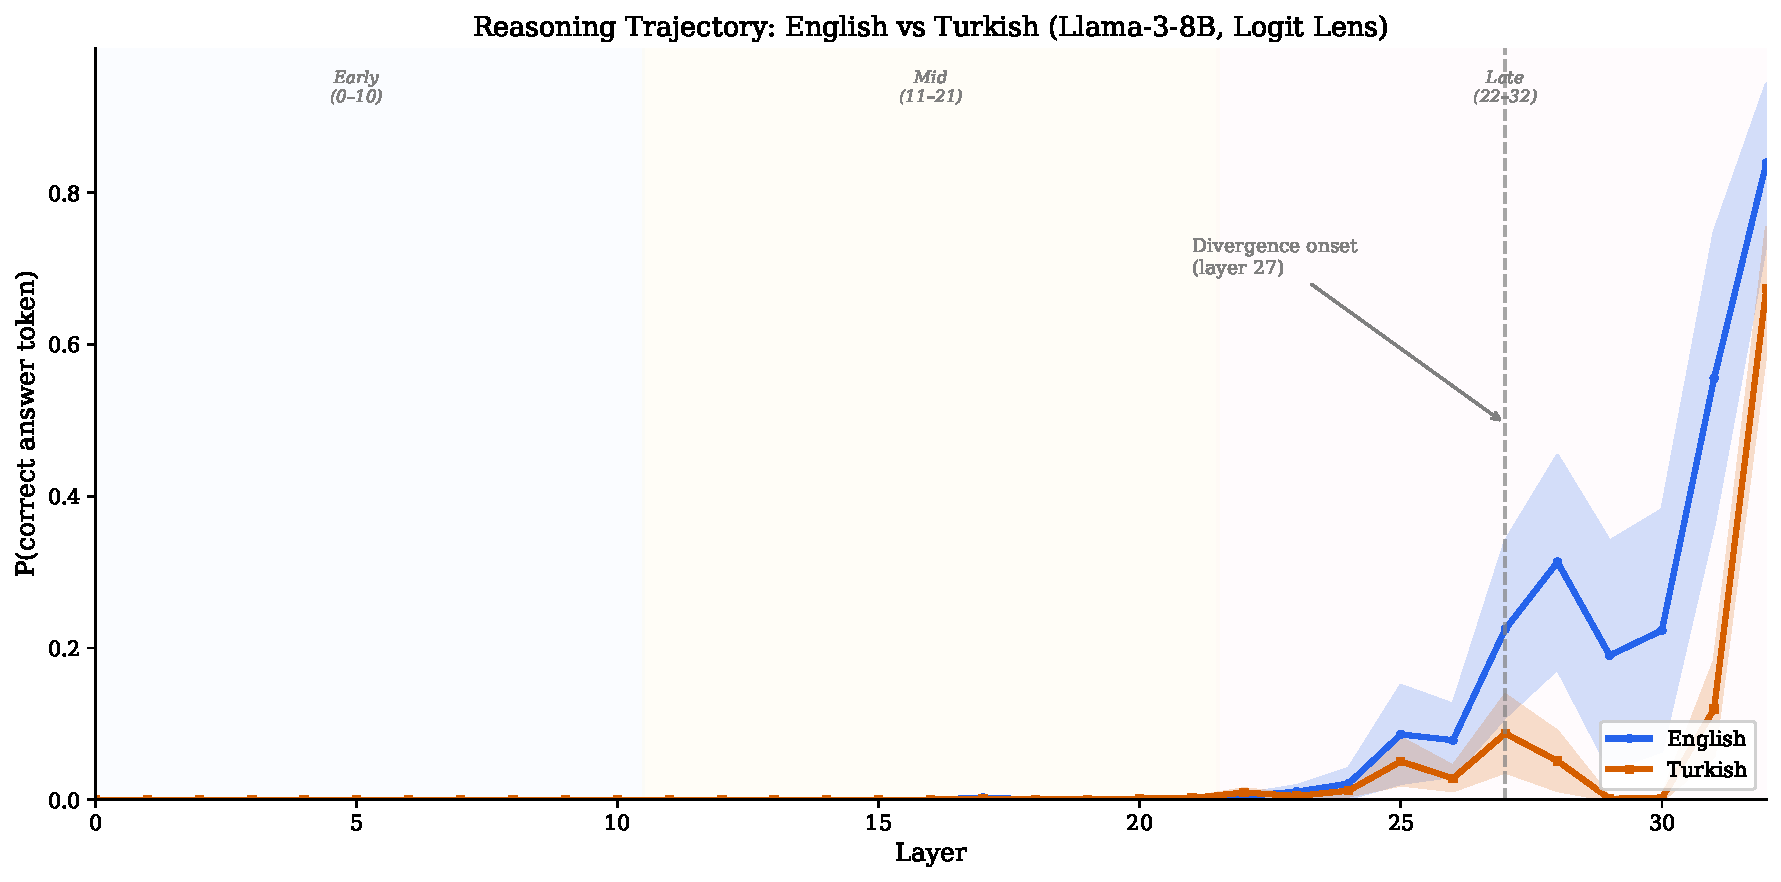
\includegraphics[width=\textwidth]{fig2_aggregate_trajectory.pdf}
    \caption{Aggregate reasoning trajectory across 15 problems. Shaded regions show 95\% CI ($t$-distribution, $n = 15$). English and Turkish track identically through mid-layers before diverging sharply in the late layers. Dashed line marks median divergence onset (layer 27).}
    \label{fig:trajectory}
\end{figure}

\subsection{Layer Region Analysis}

Table~\ref{tab:regions} quantifies the divergence by region.
The late-layer effect is large (Hedges' $g = 1.04$, corrected $p < 0.005$), while early and mid regions show negligible divergence.

\begin{table}[H]
\centering
\caption{EN--TR divergence by layer region. Exact paired permutation $p$-values with Holm--Bonferroni correction.}
\label{tab:regions}
\begin{tabular}{lcccc}
\toprule
Region & Mean $\Delta$ & Hedges' $g$ & $p$ (corrected) & Significant? \\
\midrule
Early (0--10) & $\approx 0$ & $-0.18$ & 0.673 & No \\
Mid (11--21) & $\approx 0$ & 0.26 & 0.310 & No \\
Late (22--32) & 0.17 & 1.04 & $< 0.005$ & Yes \\
\bottomrule
\end{tabular}
\end{table}

\subsection{Prompt Frame Control}

Figure~\ref{fig:frame} shows the most striking result.
When Turkish questions use a Turkish prompt frame (``Soru: \ldots Cevap:''), P(answer) drops from 0.67 to 0.12---an 82\% reduction.
The English frame is not merely a formatting choice; it is load-bearing scaffolding that enables the base model to extract Turkish answers.
This suggests the model performs cross-lingual transfer through the English prompt rather than native Turkish processing.

\begin{figure}[H]
    \centering
    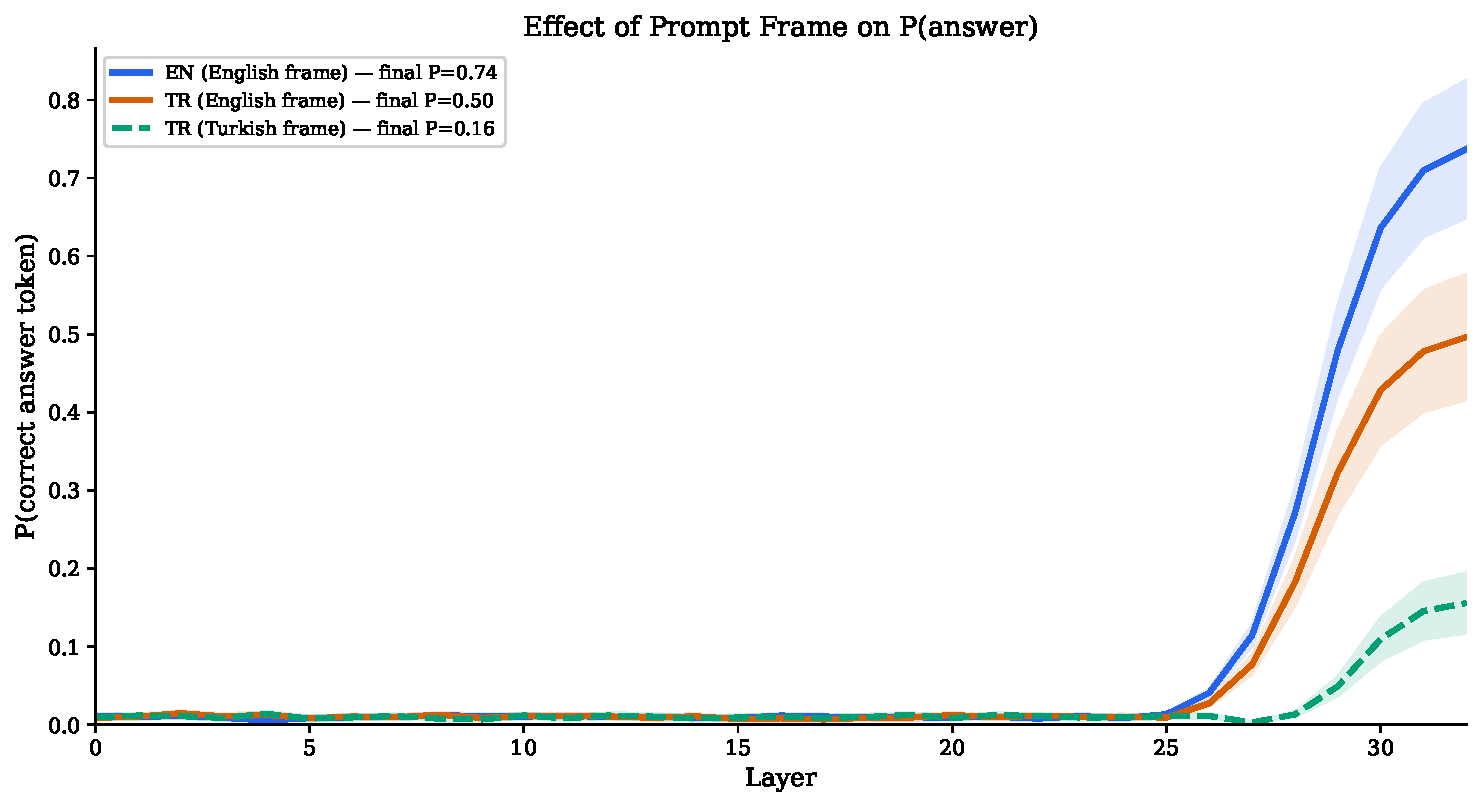
\includegraphics[width=\textwidth]{fig10_prompt_frame_control.pdf}
    \caption{Effect of prompt frame on P(correct answer). Three conditions: English question with English frame (blue), Turkish question with English frame (vermillion), and Turkish question with Turkish frame (teal, dashed). The Turkish-frame condition reveals that the model's apparent Turkish performance depends on English prompt scaffolding. Shaded bands show 95\% CI ($n = 15$).}
    \label{fig:frame}
\end{figure}

\subsection{Tokenization Confound}

Token fertility ratio correlates weakly with the P(answer) gap (Figure~\ref{fig:fertility}).
Tokenization fragmentation explains only a small fraction of the cross-lingual divergence, suggesting the gap reflects deeper processing differences, though the small sample limits statistical power.

\begin{figure}[H]
    \centering
    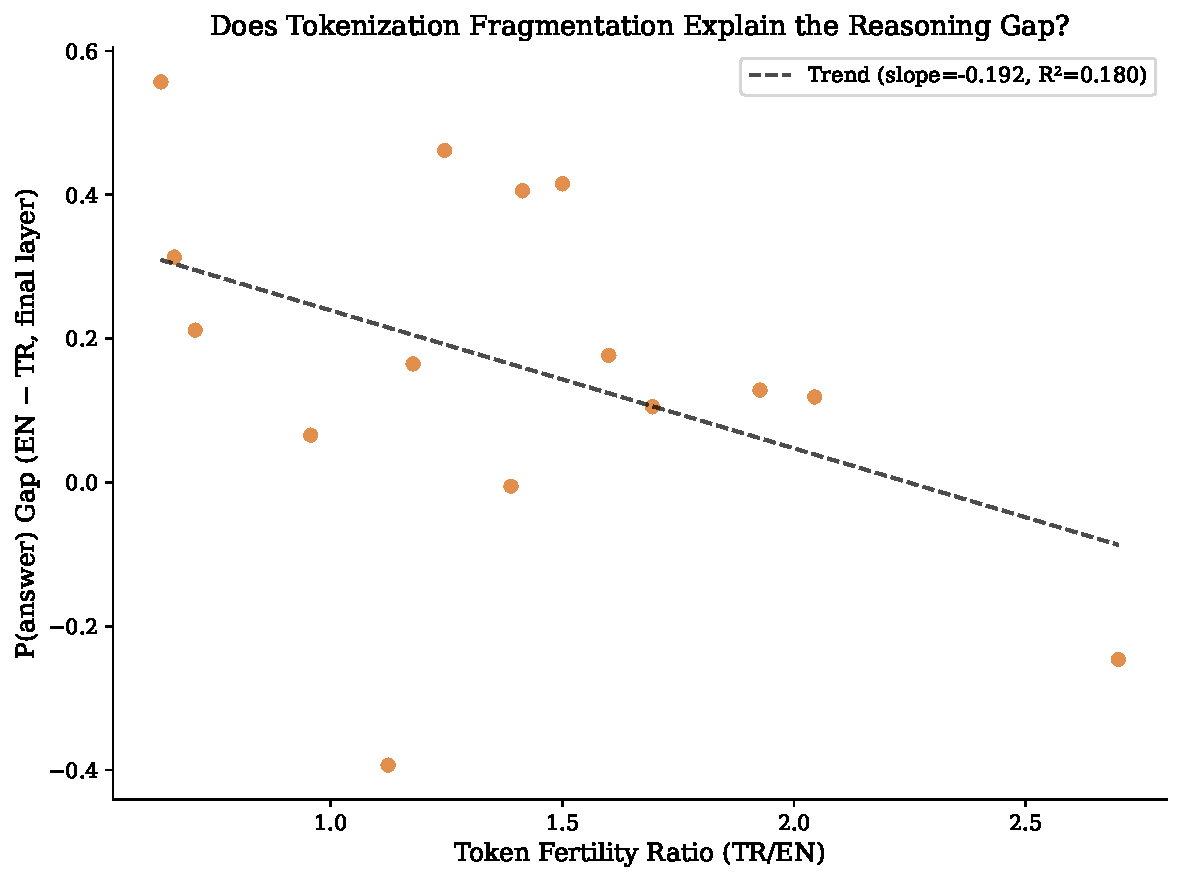
\includegraphics[width=0.65\textwidth]{fig5_fertility_vs_drop.pdf}
    \caption{Token fertility ratio vs.\ P(answer) gap with 95\% confidence band. The correlation is reported with Pearson $r$, $R^2$, and $p$-value directly on the figure. With $n = 15$, the relationship does not reach significance.}
    \label{fig:fertility}
\end{figure}

% ============================================================
\section{Discussion}
% ============================================================

\subsection{Late-Layer Divergence}

The concentration of EN--TR divergence in layers 27--32 is consistent across all 15 problems and robust to multiple analysis approaches (per-layer probability, JS divergence, entropy---see supplementary figures in the repository).
This suggests that Llama-3-8B processes mathematical content similarly across languages in its early and mid layers, with the cross-lingual gap emerging only at the output-formation stage.

This aligns with the ``English pivot'' hypothesis \citep{wendler2024}: multilingual models may route through English-like representations in intermediate layers before diverging at output.

\subsection{The English Frame Effect}

The dramatic drop when switching to a Turkish prompt frame (P = 0.67 $\rightarrow$ 0.12) is the study's most actionable finding.
It reveals that the base model's Turkish ``reasoning'' in the logit lens is substantially bootstrapped by the English frame.
This has two implications:
\begin{enumerate}[nosep]
    \item The 0.67 figure for Turkish with English frame is partly an artifact of cross-lingual transfer through the prompt, not native Turkish reasoning.
    \item The mechanism of this transfer---how the English frame helps extract Turkish answers---is itself a key research question addressable through activation patching at layers 27--32.
\end{enumerate}

\subsection{Limitations}

\begin{itemize}[nosep]
    \item \textbf{Small sample} ($n = 15$): Consistent patterns but limited statistical power. The wide confidence intervals---especially visible in Figures~\ref{fig:trajectory} and~\ref{fig:frame}---honestly communicate this limitation.
    \item \textbf{Single model}: Results may not generalize across architectures.
    \item \textbf{Logit lens linearity}: The logit lens assumes linear decodability; a tuned lens \citep{belrose2023tuned} may yield different mid-layer results.
    \item \textbf{English frame confound}: The primary analysis uses English framing for both languages. Our Turkish-frame control (Section~3.4) disentangles this partially, but full resolution requires activation patching.
    \item \textbf{First-token approximation}: Multi-token answers are tracked via their first BPE token only.
    \item \textbf{Correlational}: No causal claims without activation patching.
\end{itemize}

% ============================================================
\section{Conclusion}
% ============================================================

We demonstrate that the logit lens can precisely localize where multilingual reasoning diverges inside a language model.
For Turkish math reasoning in Llama-3-8B, the critical divergence occurs in layers 27--32, with a large effect size (Hedges' $g = 1.04$) and statistical significance after correction for multiple comparisons.
The strong dependence on the English prompt frame suggests that the model's cross-lingual transfer mechanism is itself a promising target for mechanistic analysis.

These findings identify specific layers for activation patching interventions and validate the feasibility of the diagnostic approach for studying multilingual reasoning at a mechanistic level.

% ============================================================
\bibliographystyle{apalike}

\begin{thebibliography}{99}

\bibitem[Belrose et al., 2023]{belrose2023tuned}
Belrose, N., Furman, H., Smith, L., Halawi, D., Oesterling, I., Wright, L., \& Steinhardt, J. (2023).
Eliciting Latent Predictions from Transformers with the Tuned Lens.
\textit{arXiv:2303.08112}.

\bibitem[Cobbe et al., 2021]{cobbe2021gsm8k}
Cobbe, K., Kosaraju, V., Bavarian, M., Chen, M., Jun, H., Kaiser, L., \ldots \& Schulman, J. (2021).
Training Verifiers to Solve Math Word Problems.
\textit{arXiv:2110.14168}.

\bibitem[Ismayilzada et al., 2025]{ismayilzada2025}
Ismayilzada, E., et al. (2025).
Evaluating Morphological Compositional Generalization in Large Language Models.
\textit{NAACL 2025}. arXiv:2410.12656.

\bibitem[Liu et al., 2026]{liu2026multilingual}
Liu, Q., et al. (2026).
Large Reasoning Models Are (Not Yet) Multilingual Latent Reasoners.
\textit{arXiv:2601.02996}.

\bibitem[nostalgebraist, 2020]{nostalgebraist2020}
nostalgebraist (2020).
Interpreting GPT: The Logit Lens.
\textit{LessWrong}.

\bibitem[Wendler et al., 2024]{wendler2024}
Wendler, C., Veselovsky, V., Monea, G., \& West, R. (2024).
Do Llamas Work in English? On the Latent Language of Multilingual Transformers.
\textit{ACL 2024}. arXiv:2402.10588.

\bibitem[Yuksel et al., 2024]{yuksel2024turkishmlu}
Yuksel, O., et al. (2024).
TurkishMMLU: Measuring Massive Multitask Language Understanding in Turkish.
\textit{Findings of EMNLP 2024}. arXiv:2407.12402.

\end{thebibliography}

\end{document}
